\chapter{Implementación}

\section{Stack Tecnológico}
\begin{itemize}
    \item Ubuntu 22.04/24.04 LTS en USB bootable.
    \item \texttt{iw} y \texttt{ip} para configuración IBSS.
    \item Python 3 + Flask para el daemon y API web.
    \item ffmpeg para codificación y streaming UDP/MPEG-TS.
    \item mpv / ffplay para reproducción.
    \item systemd para autoarranque.
\end{itemize}

\section{Servicios systemd}
El servicio \texttt{adhoc-node.service} se habilita con \texttt{systemctl enable} y ejecuta \texttt{init-node.sh} al boot. Este script configura la red y lanza el daemon Python.

\section{Elección de Master}
Se calcula un \textit{score} basado en RAM libre, núcleos de CPU y carga del sistema. Los nodos intercambian scores vía heartbeats UDP broadcast/multicast. El nodo con mayor score dentro de la celda se declara Master.

\section{Diagrama de Clases}
\begin{figure}[h]
\centering
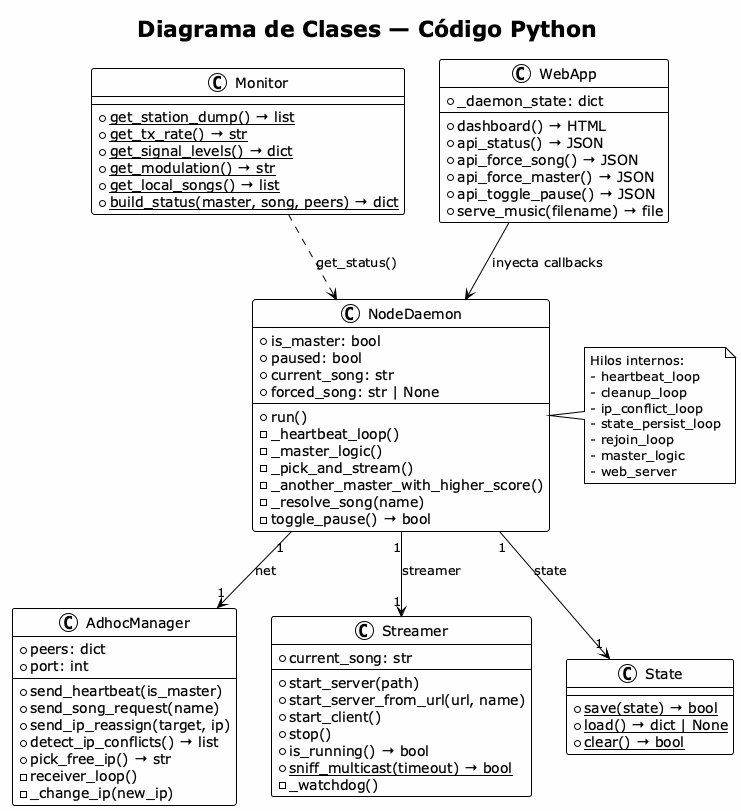
\includegraphics[width=\textwidth]{diagrams/class-diagram.png}
\caption{Clases Python principales y sus relaciones.}
\label{fig:classes}
\end{figure}

\section{Secuencia de Streaming}
\begin{figure}[h]
\centering
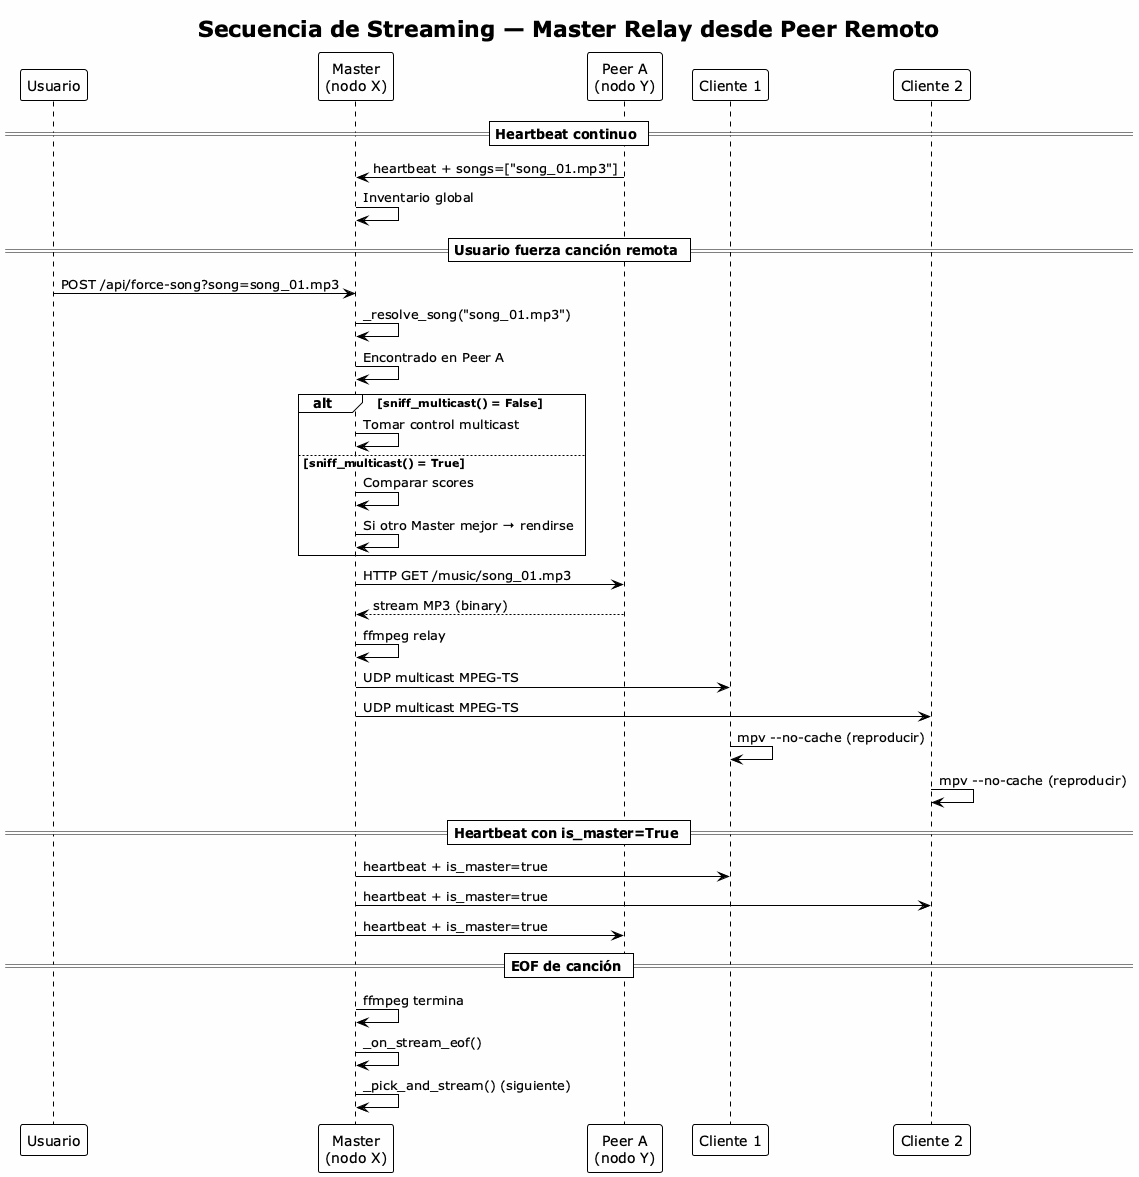
\includegraphics[width=\textwidth]{diagrams/streaming-sequence.png}
\caption{Flujo de relay HTTP → ffmpeg → multicast UDP.}
\label{fig:streaming}
\end{figure}

\section{Transición de Master}
\begin{figure}[h]
\centering
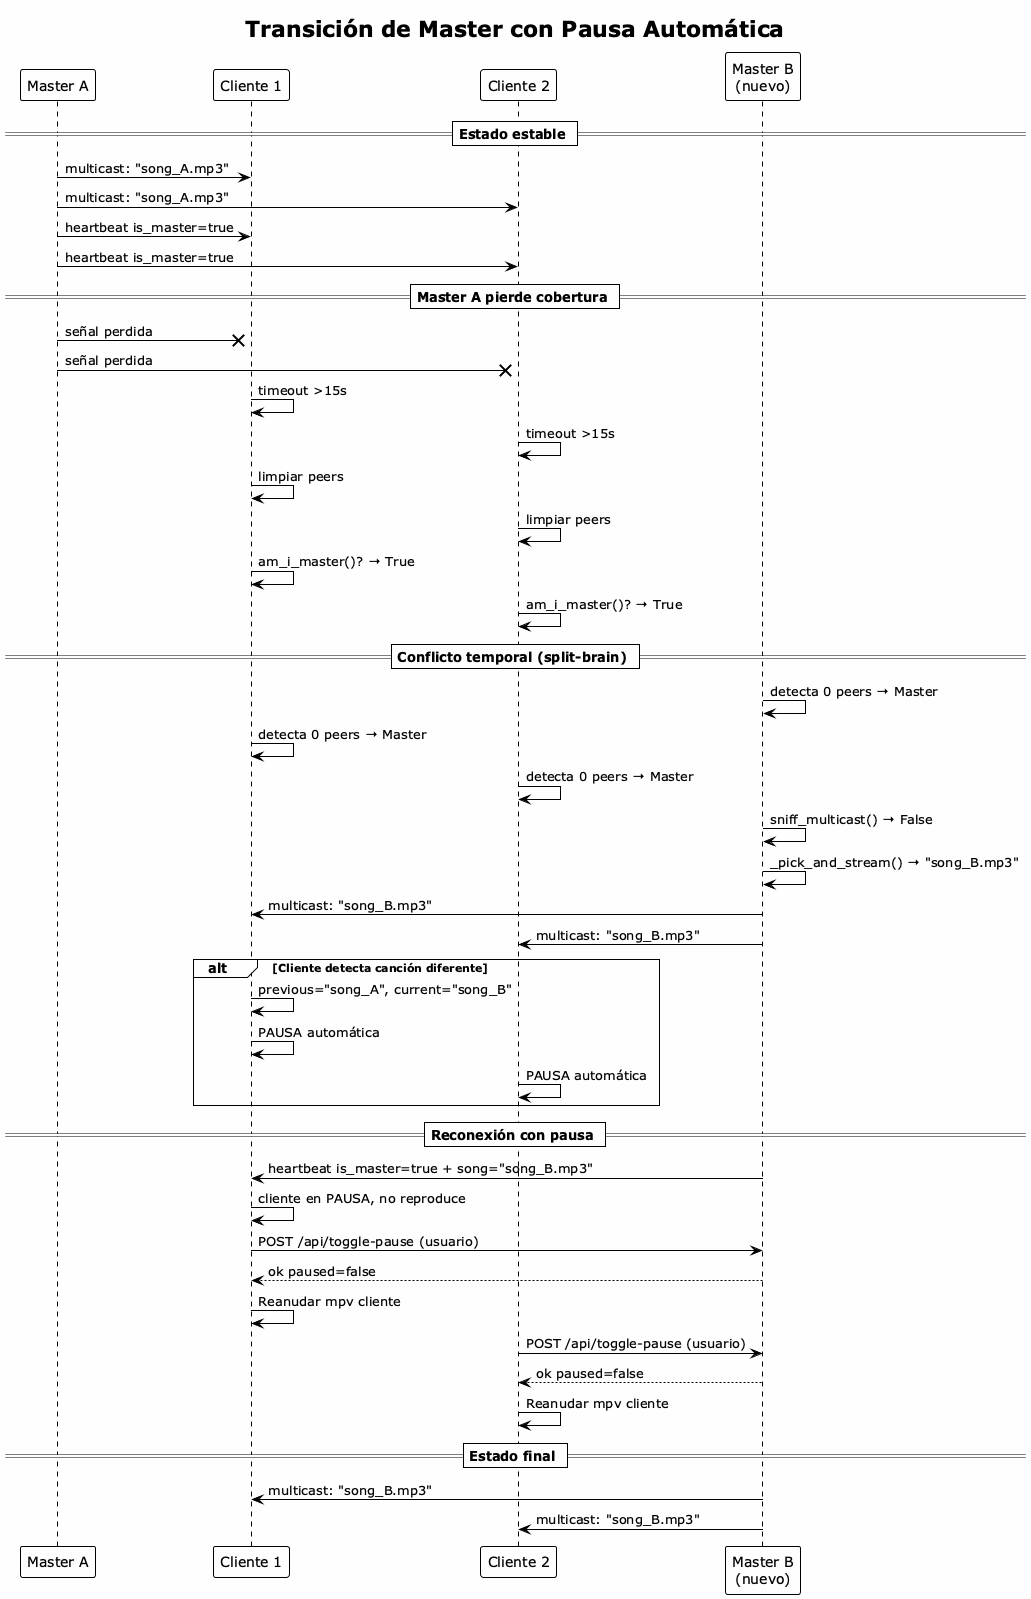
\includegraphics[width=\textwidth]{diagrams/master-transition.png}
\caption{Split-brain, pausa automática y reanudación por el usuario.}
\label{fig:transition}
\end{figure}

\section{Estados de Pérdida}
\begin{figure}[h]
\centering
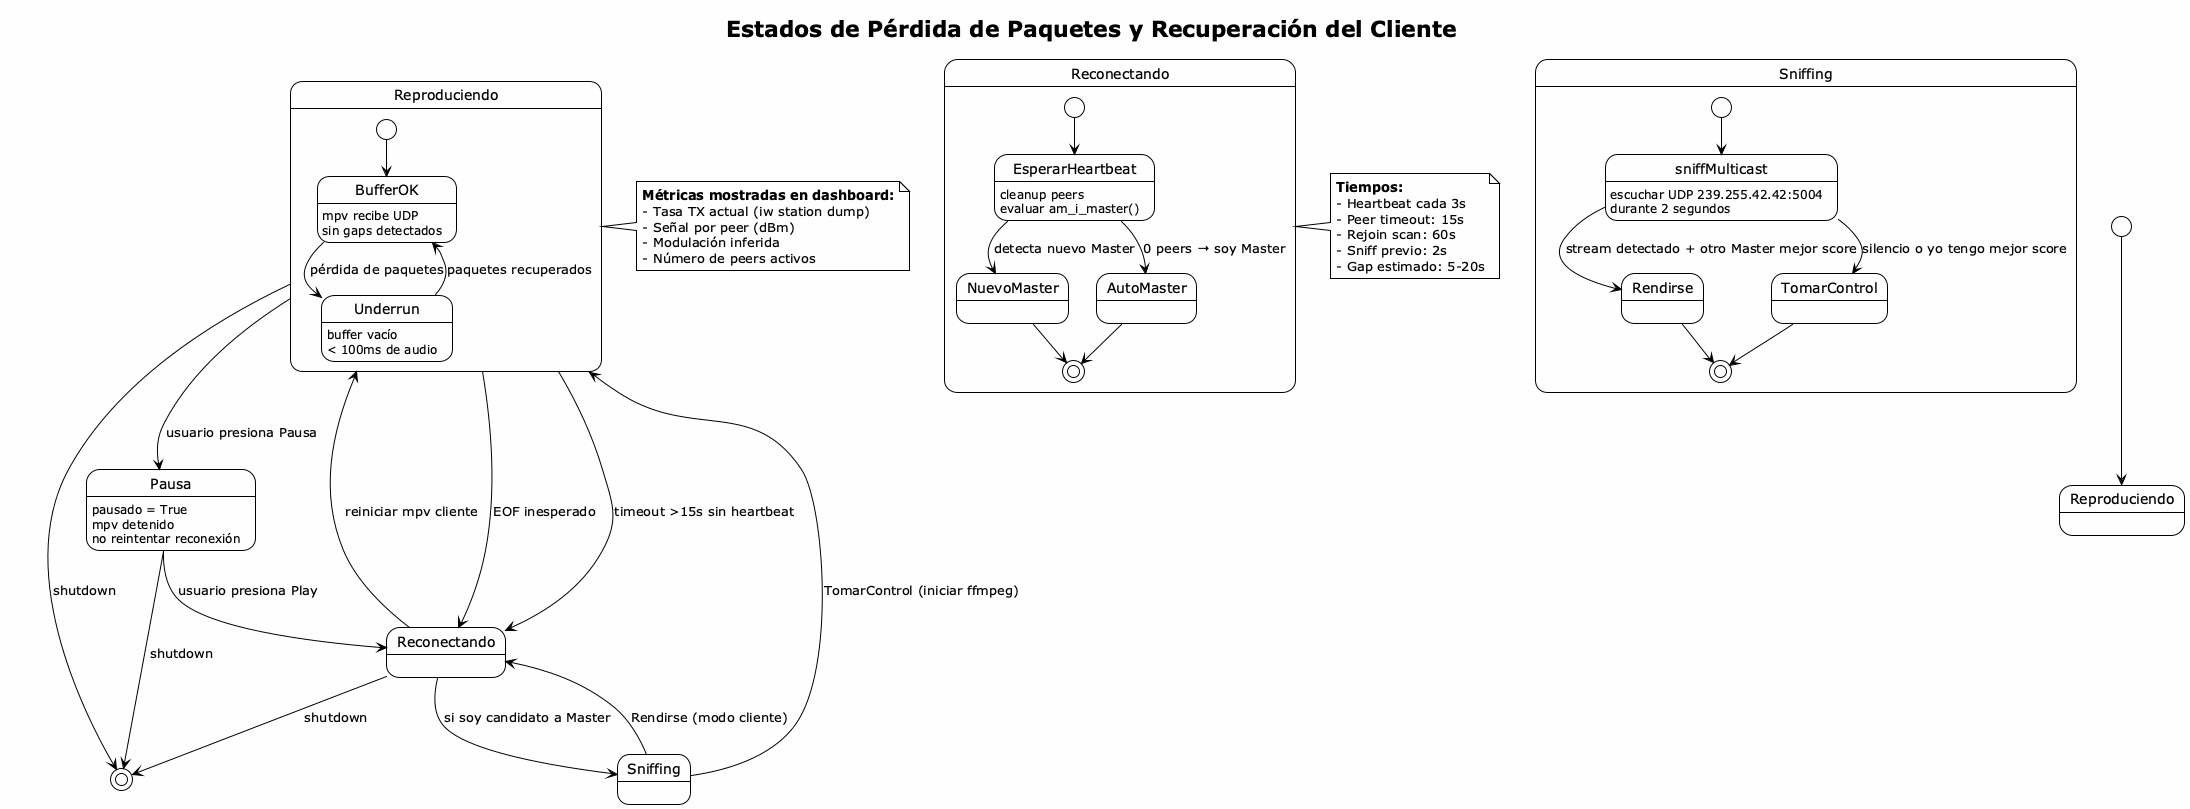
\includegraphics[width=\textwidth]{diagrams/packet-loss-recovery.png}
\caption{Máquina de estados: reproducción, pausa, reconexión y sniffing.}
\label{fig:packetloss}
\end{figure}

\section{Indicadores}
El panel web en \texttt{http://<nodo>:8080} muestra:
\begin{itemize}
    \item Tasa de transmisión activa (\texttt{iw station dump}).
    \item Nodos activos y nivel de señal por peer.
    \item Modulación inferida del bitrate reportado.
    \item Canciones locales y canción en streaming.
    \item Estado de pausa/play.
\end{itemize}
